\chapter{Experimentos numéricos}
\label{cap4}

\section{Modelo utilizado e aquisição}

 Os testes foram feitos utilizando um modelo com 9000 $m$ de comprimento e 3000 $m$ de profundidade. Quanto ao modelo de velocidade, foi utilizado o \textit{Marmousi} suavizado (Fig. \ref{fig:marmousi}). O modelo usado na Figura \ref{fig:modelortm} serviu para utilizar como entrada para o RTM. Foram utilizados 240 tiros nesse processo. O modelo utilizado para fazer a modelagem e o imageamento foi \textit{Intel(R) Core(TM) i5-7200U CPU 2.50GHz}, cujo possui 4 threads físicos.
 
 \begin{figure}[ht!]
	\centering
	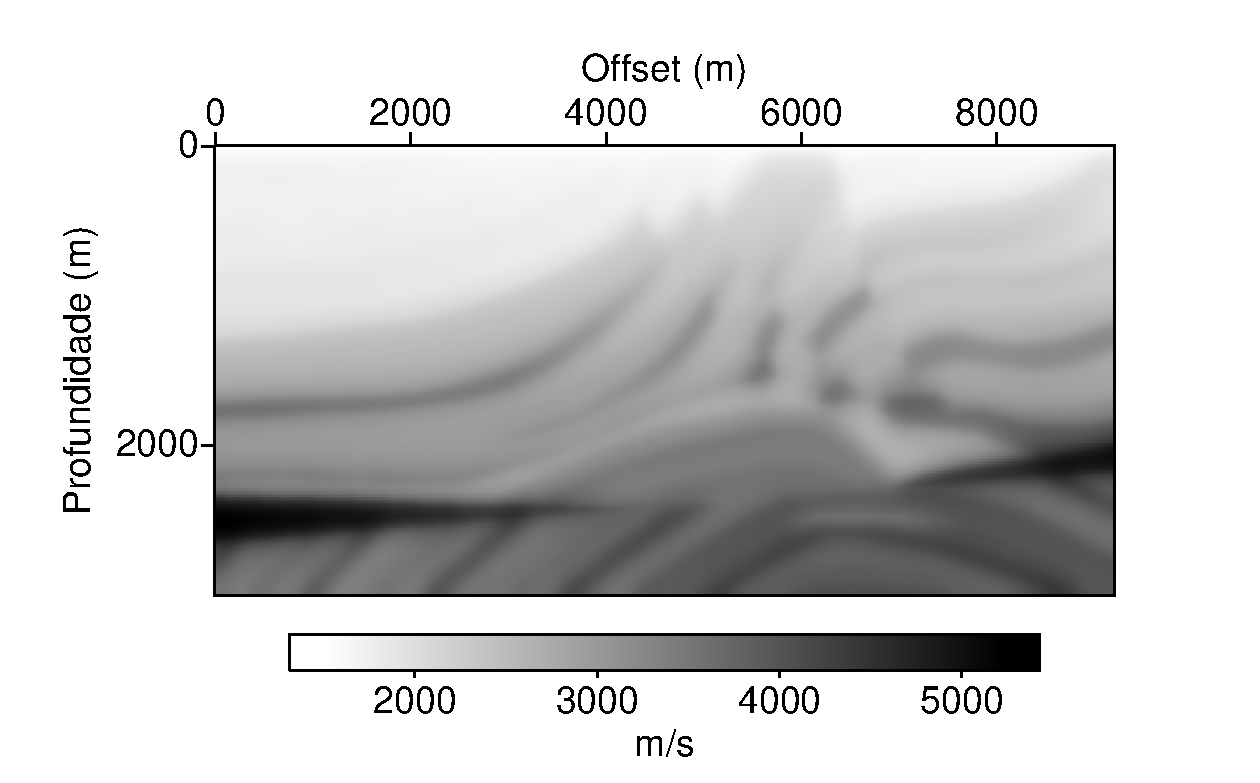
\includegraphics[width=15cm]{marmousi}
	\caption{Modelo de velocidade utilizado para a modelagem direta: modelo de Marmousi suavizado.} \label{fig:marmousi}
\end{figure} 
\begin{figure}[ht!]
	\centering
	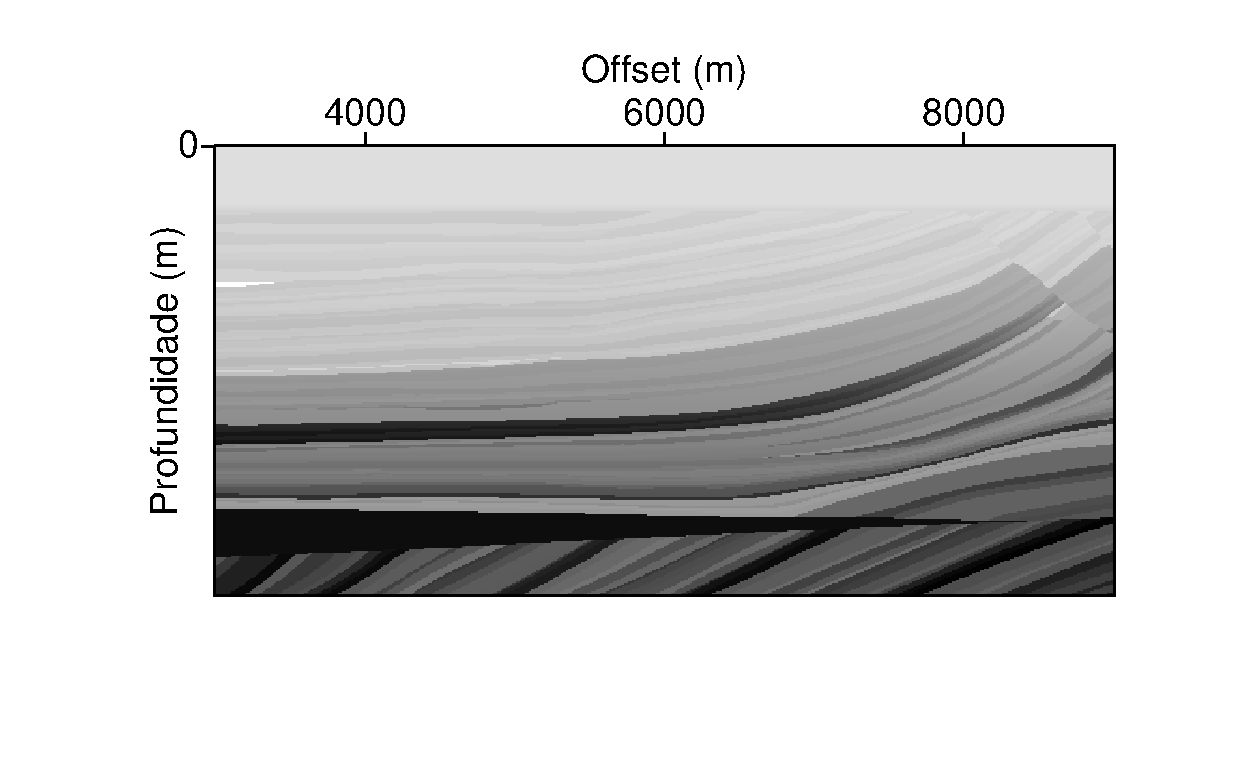
\includegraphics[width=15cm]{modelortm}
	\caption{Modelo utilizado para fazer a migração.} \label{fig:modelortm}
\end{figure} 
 \section{Resultados e discussões}
 
 Após feito o processo de modelagem e aplicado o RTM, foi gerada a Figura \ref{fig:rtm}. 
 \begin{figure}[ht!]
 	\centering
 	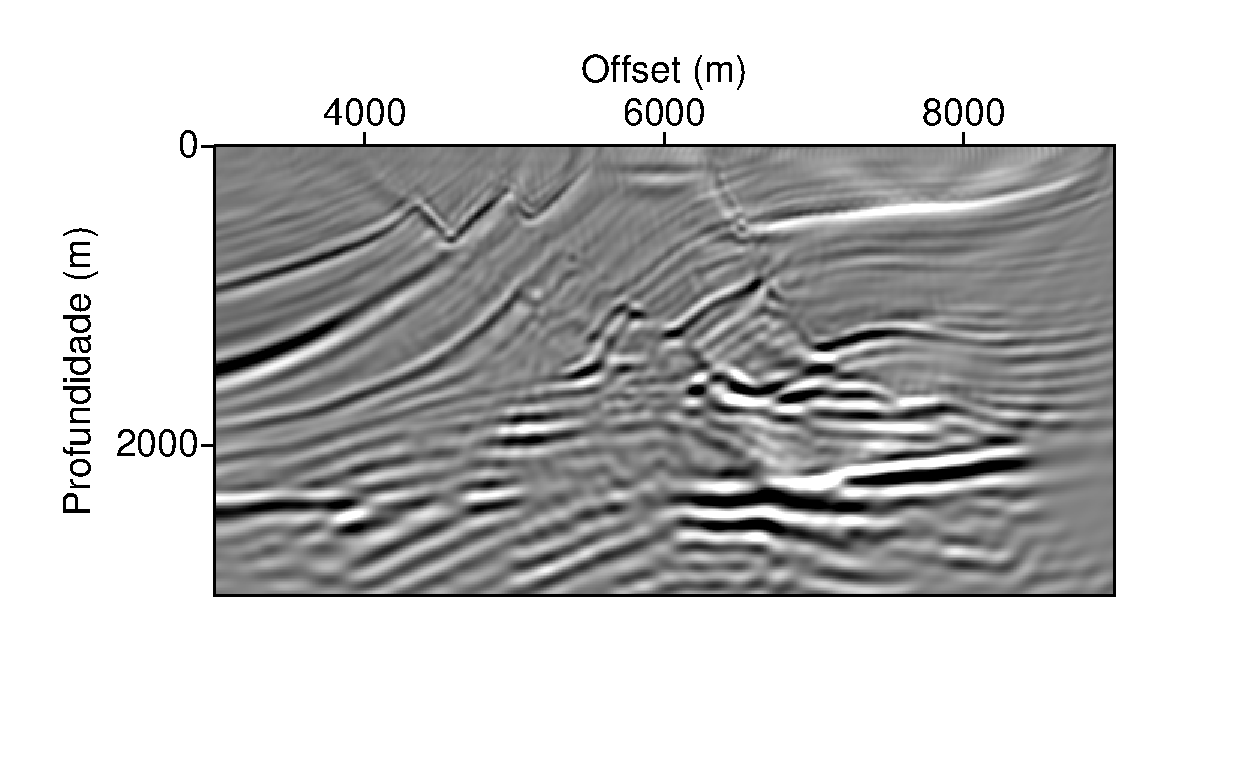
\includegraphics[width=15cm]{rtmfinal}
 	\caption{Imagem migrada do modelo de Marmousi filtrada.} \label{fig:rtm}
 \end{figure} 
 Na Figura \ref{fig:rtm}, nota-se que os eventos estão bem destacados, sem a presença de reflexões. Portanto, é possível analisar que esta técnica de imageamento teve bom funcionamento.
 
  Quanto ao custo computacional do RTM, foram necessárias aproximadamente 80 horas para gerar a Figura \ref{fig:rtm}. Caso não houvesse sido utilizada a paralelização, a tendencia era de maior custo computacional.








